\section{Приложение}
\subsection{Приложение 1} \label{Приложение 1}
Схема экспериментальной установки приведена на рис. 1.
\begin{figure}[ht]
    \label{figure1}
    \center{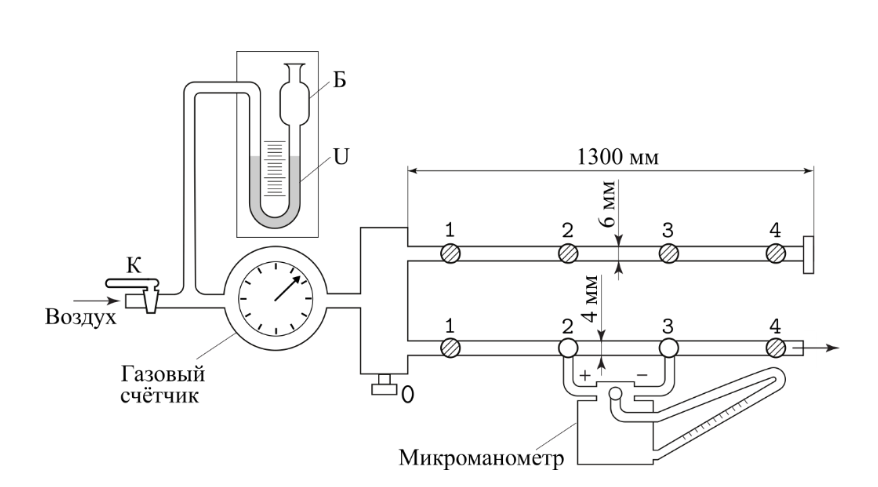
\includegraphics[scale=0.4]{img/exp_ust.png}}
    \caption{Экспериментальная установка для измерения коэффициента вязкости воздуха}
\end{figure}

Поток воздуха под давлением, немного превышающим атмосферное, поступает через газовый счетчик в тонкие металлические трубки. Воздух нагнетается компрессором, интенсивность его подачи регулируется краном К. Трубки снабжены заглушками на концах и рядом миллиметровых отверстий, к которым можно подключать микроманометр. В рабочем состоянии открыта заглушка на одной рабочей трубке, микроманометр подключен к двум её выводам, остальные отверстия закрыты. 

Перед входом в газовый счетчик установлен U-образный манометр. Он служит для измерения давления газа на входе в счётчик, а также предохраняет его от выхода из строя. При превышении максимального избыточного давления на входе счетчика (30 см. вод. ст) вода выплескивается из трубки в защитный баллон Б.
\newpage
\subsection{Приложение 2} \label{Приложение 2}
Схема устройства микроманометра приведена на рис. 2.
\begin{figure}[ht]
    \label{figure2}
    \center{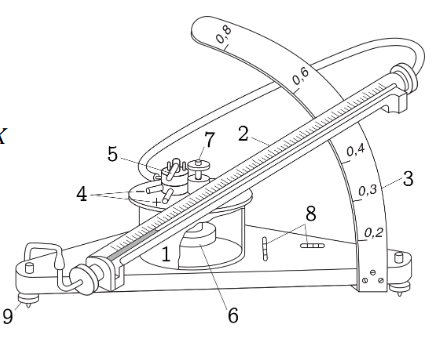
\includegraphics[scale=0.5]{img/micro.png}}
    \caption{Жидкостный микроманометр ММН-2400}
\end{figure}

\textbf{Устройство}
\begin{itemize}
    \item[1] 
    Сосуд с рабочей жидкостью
    \item[2]
    Измерительная шкала
    \item[3]
    Стойка для регулировки наклона
    \item[4]
    Место крепления измерительных трубок
    \item[5] 
    Переключатель режима работы
    \item[6] 
    Поплавок регулировки уровня спирта (для установки нуля)
    \item[7] 
    Винт, регулирующий глубину погружения поплавка
    \item[8] 
    Индикаторы горизонтального уровня
    \item[9] 
    Регулируемые ножки
\end{itemize}

Разность давлений на входах манометра измеряется по высоте подъёма рабочей жидкости. Регулировка
наклона позволяет измерять давление в различных диапазонах. На крышке прибора установлен трехходовый кран, имеющий два рабочих положения - (0) и (+). В положении (0) производится установка мениска жидкости на ноль, что необходимо сделать перед началом работы. В положении (+) производятся измерения.

\textbf{Измерения}

Связь измеряемого давления $P$ с отсчётом делений по шкале $N$
\[ P[\text{мм. вод. ст.}] = N\cdot K\cdot n\]
или
\[P[\text{Па}] = 9.81\cdot N\cdot K\cdot n\]
где $K = 0.2, 0.4, 0.6, 0.8$ - угловой коэффициент наклона трубки микроманометра, $n$ - поправочный множитель, учитывающий отличие плотности залитого спирта от $0.8095\frac{\text{г}}{\text{см}^3}$.
\begin{table}[h]
    \centering
    \begin{tabular}{|c|c|c|c|c|c|c|c|c|c|}
    \hline
    $t, \celsius$ & 16 & 18 & 20 & 22 & 24 & 26 & 28 & 30 &32 \\ \hline
     $\rho, \frac{\text{г}}{\text{см}^3}$ & 0,8109  & 0,8092   & 0,8075   & 0,8057   & 0,8040 & 0,8022 & 0,8004 & 0,7987 & 0,7969 \\ \hline
     $n, \text{отн. ед.}$ & 1,0018 & 0,9996 & 0,9975 & 0,9953 & 0,9932 & 0,9910 & 0,9888 & 0,9866 & 0,9844 \\ \hline
     
\end{tabular}
    \caption{Зависимость плотности 96\% спирта от температуры}
    \label{tab:t1}
\end{table}

\subsection{Приложение 3} \label{Приложение 3}
Схема устройства газового счетчика приведена на рис. 3.
\begin{figure}[ht]
    \label{figure3}
    \center{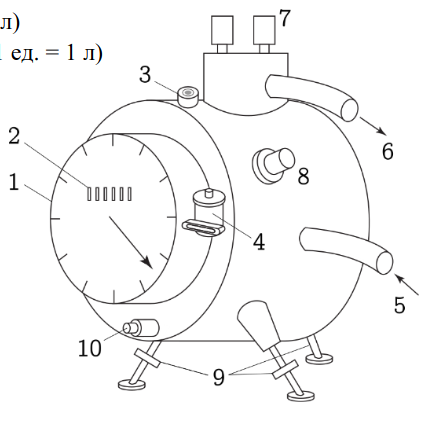
\includegraphics[scale=0.5]{img/schet.png}}
    \caption{Газовы счетчик}
\end{figure}

\textbf{Устройство}
\begin{itemize}
    \item[1] 
    Измерительная шкала (1 оборот = 5 л)
    \item[2]
    Счётно-суммирующее устройство (1 ед. = 1 л)
    \item[3]
    Индикатор горизонтального уровня
    \item[4]
    Водомерное устройство
    \item[5] 
    Трубка для подачи газа
    \item[6] 
    Трубка для отвода газа
    \item[7] 
    Патрубки для подключения внешнего манометра
    \item[8] 
    Место установки термометра
    \item[9] 
    Регулируемые ножки
    \item[10]
    Сливное отверстие
\end{itemize}

\textbf{Характеристики}
\begin{itemize}
    \item 
    Класс точности: 1.0
    \item
    Пределы измерения расхода: от $20 \frac{\text{л}}{\text{ч}}$ до $1000 \frac{\text{л}}{\text{ч}}$
    \item
    Цена наименьшего деления: 0,02 л
    \item
    Предел измерения стрелочного механизма (1 оборот): 5 л
    \item
    Максимально допустимый перепад давления: 600 мм вод. ст. (5885 Па)
\end{itemize}

Работа счётчика основана на принципе вытеснения: на цилиндрической ёмкости жёстко укреплены лёгкие чаши (см. Рис. 4, где для упрощения изображены только две чаши), в которые поочередно поступает воздух из входной трубки расходомера. Когда чаша наполняется, она всплывает и её место занимает следующая и т.д. Вращение оси передаётся на счётно-суммирующее устройство.

\begin{figure}[ht]
    \label{figure4}
    \center{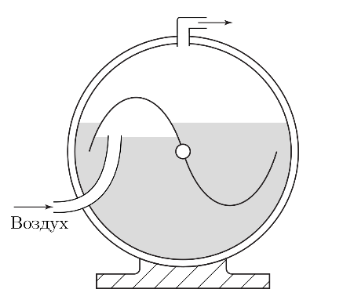
\includegraphics[scale=0.5]{img/schet2.png}}
    \caption{Принцип работы барабанного газосчетчика}
\end{figure}
\newpage
\subsection{Приложениние 4} \label{Приложение 4}
\begin{table}[ht]
\begin{tabular}{|c|c|c|}
\hline
{$\Delta P$, дел} & {$\Delta P$, Па} & {$Q$, л/мин} \\
\hline
10 & 19.61 & 0.6 \\ \hline
20 & 39.23 & 1.4 \\ \hline
30 & 58.84 & 2.1 \\ \hline
40 & 78.45 & 2.8 \\ \hline
50 & 98.07 & 3.6 \\ \hline
60 & 117.68 & 4.2 \\ \hline
70 & 137.29 & 4.9 \\ \hline
76 & 149.06 & 5.3 \\ \hline
80 & 156.91 & 5.4 \\ \hline
90 & 176.52 & 5.7 \\ \hline
100 & 196.13 & 5.8 \\ \hline
110 & 215.75 & 6 \\ \hline
120 & 235.36 & 6.2 \\ \hline
150 & 294.20 & 6.8 \\ \hline
200 & 392.27 & 7.7 \\ \hline
240 & 470.72 & 8.4 \\ \hline
\end{tabular}
\caption{
\centering Зависимость расхода $Q$ от перепада давления $\Delta P$ для трубки диаметром d = 3.95 мм.}
\end{table}

\begin{table}[ht]
\begin{tabular}{|c|c|c|}
 \hline
{$\Delta P$, дел} & {$\Delta P$, Па} & {$Q$, л/мин} \\
 \hline
4 & 7.85 & 0.7 \\  \hline
8 & 15.69 & 1.6 \\ \hline
12 & 23.54 & 2.7 \\ \hline
16 & 31.38 & 3.4 \\ \hline
20 & 39.23 & 4.4 \\ \hline
24 & 47.07 & 5.3 \\ \hline
28 & 54.92 & 6.0 \\ \hline
32 & 62.76 & 6.7 \\ \hline
40 & 78.45 & 7.6 \\ \hline
80 & 156.91 & 10.1 \\ \hline
100 & 196.13 & 11.4 \\ \hline
120 & 235.36 & 12.7 \\ \hline
140 & 274.59 & 13.7 \\ \hline
160 & 313.81 & 14.9 \\ \hline
170 & 333.43 & 16.0 \\ \hline
\end{tabular}
\caption{
\centering Зависимость расхода $Q$ от перепада давления $\Delta P$ для трубки диаметром d = 5.05 мм.}
\end{table}
\newpage
\subsection{Приложениние 5} \label{Приложение 5}

Из выражения \eqref{eq: Re} и уравнения Менделеева-Клапейрона следует, что
\begin{equation}
    Re_\text{кр} = \frac{\rho u a}{\eta} = \frac{p\mu}{RT} \frac{Q_\text{кр}}{\pi r^2}\cdot \frac{r}{\eta} \label{eq: Re_kr}
\end{equation}
где в качестве характерной скорости использована средняя скорость потока воздуха $u = \frac{Q_\text{кр}}{\pi r^2}$, и радиус трубки $r$ использован как характерный размер. 
Из \eqref{eq: Re_kr} следует, что
\begin{equation}
    Q_\text{кр} = \frac{Re_\text{кр}\cdot RT\cdot \pi r\eta}{p\mu} \label{eq: Q_kr}
\end{equation}

\subsection{Приложениние 6} \label{Приложение 6}

\begin{table}[ht]
\begin{tabular}{|c|c|}
 \hline
$P_0-P, \text{Па}$ & $x, \text{м}$ \\
 \hline
$102 \pm 2$ & $1.31 \pm 0.01$  \\  \hline
$79\pm 2$ & $1.20 \pm 0.01$ \\ \hline
$67\pm 2$ & $0.81\pm 0.01$  \\ \hline
$59\pm 2$ & $0.70\pm 0.01$  \\ \hline
$47\pm 2$ & $0.50\pm 0.01$  \\ \hline
$37\pm 2$ & $0.41\pm 0.01$  \\ \hline
$33\pm 2$ & $0.40\pm 0.01$  \\ \hline
$20\pm 2$ & $0.30\pm 0.01$  \\ \hline
$14\pm 2$ & $0.11\pm 0.01$  \\ \hline
\end{tabular}
\caption{Зависимость разности $P-P_0$ давления в трубке на расстоянии $x$ и давления на входе в трубку от расстояния $x$ до входа в трубке диаметром $d = 3.95\text{мм}$}
\end{table}

\begin{table}[ht]
\begin{tabular}{|c|c|}
 \hline
$P_0-P, \text{Па}$ & $x, \text{м}$ \\
 \hline
$49 \pm 2$ & $1.31\pm 0.01$  \\  \hline
$45\pm 2$ & $1.20 \pm 0.01$ \\ \hline
$37\pm 2$ & $0.81\pm 0.01$  \\ \hline
$33\pm 2$ & $0.70\pm 0.01$  \\ \hline
$30\pm 2$ & $0.50\pm 0.01$  \\ \hline
$21\pm 2$ & $0.41\pm 0.01$  \\ \hline
$20\pm 2$ & $0.40\pm 0.01$  \\ \hline
$10\pm 2$ & $0.30\pm 0.01$  \\ \hline
$7\pm 2$ & $0.11\pm 0.01$  \\ \hline
\end{tabular}
\caption{Зависимость разности $P-P_0$ давления в трубке на расстоянии $x$ и давления на входе в трубку от расстояния $x$ до входа в трубке диаметром $d = 3.95\text{мм}$}
\end{table}

\subsection{Приложениние 7} \label{Приложение 7}

\begin{table}[ht]
\begin{tabular}{|c|c|}
 \hline
$t, \celsius$ & $\eta\cdot 10^{-5}, \text{Па}\cdot\text{с}$ \\
 \hline
$-50$ & $1.58$  \\  \hline
$-20$ & $1.63$ \\ \hline
$0$ & $1.72$  \\ \hline
$20$ & $1.81$  \\ \hline
$25$ & $1.84$  \\ \hline
$50$ & $1.96$  \\ \hline
$100$ & $2.18$  \\ \hline
$200$ & $2.58$  \\ \hline
$400$ & $3.28$  \\ \hline
\end{tabular}
\caption{Зависимость динамической вязкости $\eta$ воздуха от температуры $t$}
\end{table}